\chapter{肝 大}

\section{【如何确定肝大】}

如成年人仰卧和侧卧位吸气时,可触及肝脏称肝大(hepatomegaly)。肝脏的触诊和叩诊是检查肝脏增大的重要临床方法。正常成年人肝脏上界一般在右锁骨中线第5肋间,下界在肋缘下大多不可扪及。正常情况下肝右叶下缘在剑突下2~3cm,但由于被腹直肌掩盖,常不易扪及。正常肝脏大小为25cm(长径)×15cm(上下径)×16cm(前后径)。

影响肝脏触诊结果的因素颇多。5岁以下儿童、少数正常成人尤其青年人、瘦长体型、多孕妇女在深吸气时,肋缘下1~2cm可触及到肝脏,边缘锐利,质软,无压痛。多饮水、饭后及运动后肝脏也可暂时性增大。在肺气肿、右胸腔大量积液、膈下脓肿、严重胸廓畸形时,肝脏因位置下移也可触及。病理性肝大除根据可触及肝脏外,还要了解其形态、质地、表面及边缘情况、有无压痛及叩痛,以及其他检查结果来确定。

病理性肝大质地多不正常,表面不光滑,有压痛。大小可分轻度(肋下触及1~3cm)、中度(肋下3~5cm)、重度(平脐)。肝脏的硬度通常也可区分为三度:一度(Ⅰ°),质柔软,触诊时有如指按口唇的硬度,这是正常肝脏的硬度;二度(Ⅱ°),略硬,有如指按鼻尖的硬度,一般见于各期肝炎、肝脓肿、血吸虫病、脂肪肝等;三度(Ⅲ°),硬度明显增加,有如指按两眉之间的硬度,可见于慢性肝炎、肝硬化、晚期血吸虫病、恶性肿瘤等。按病变范围可分为弥漫性和局限性肝大,前者由于普遍性肝脏病变所致,后者由于肝内占位性病变如肿瘤、脓肿、囊肿等所致。

\section{【肝大的诊断步骤】}

临床上对已发现的肝脏肿大,首先要判断是否为病理性,体格检查要注意了解肝脏的质地、表面与边缘情况,有无触痛、压痛及叩击痛,以及某些特殊表现如波动感、搏动、震颤等,并结合其他临床表现与实验室检查资料加以全面分析。

临床诊断时大致有两种思路:一是先将其分为感染性与非感染性疾病,再将其分为几个亚类,逐步缩小、过滤具体到某一种疾病;另一种思路是根据突出的伴随症状或体征与疾病的关联性确定诊断方向,再逐一鉴别筛查。临床上一般可两种思路交叉、综合应用。

\subsection{(一)病史采集要点}

\subsubsection{1.病史资料}

流行病史常能为肝大提供诊断线索。患者是否来自血吸虫病、包虫病(棘球蚴病)、疟疾、黑热病流行地区;有无进食生鱼;有无输血、注射史。肝硬化患者往往有肝炎、黄疸、慢性乙醇性中毒等病史。

\subsubsection{2.伴随症状}

\paragraph{(1)发热:}

急性病毒性肝炎起病时常有短暂低度发热。细菌性感染如细菌性肝脓肿、化脓性胆管炎、胆囊炎常有寒战、高热、伴明显毒血症。原发性肝癌多数不热或仅有低热,少数亦可有持续高热或周期性发热,肝结核、肝结节病、肉芽肿性肝炎可有长期低热。

\paragraph{(2)肝区疼痛:}

病毒性肝炎引起者多为隐痛。肝脓肿、肝癌可有剧烈而持续的痛。胆囊炎、胆管炎的疼痛常为阵发性。

\paragraph{(3)黄疸:}

出现于发热、乏力和消化道症状数天后者,为黄疸型病毒性肝炎典型表现。胆石症、肿瘤引起明显胆道梗阻压迫时,黄疸为主要症状。胆石引起的黄疸常在腹痛后迅速出现,如梗阻缓解,黄疸可迅速消退。

\subsection{(二)体格检查重点}

\subsubsection{1.肝}

对肝大要注意其程度、形态、质地、表面状态,有无压痛、叩痛、波动或搏动等。

\subsubsection{2.注意有无肝硬化特有征象}

如皮肤色素沉着、蜘蛛痣、肝掌、男性乳房发育、睾丸萎缩、杵状指等。门脉高压症如腹壁静脉曲张、脾大、腹水等。

\subsubsection{3.皮肤改变}

皮肤的色素、瘙痒抓痕、紫癜、黄疸等。

\subsubsection{4.心脏检查}

有无心率增速、杂音、心音遥远以及有无颈静脉怒张、气急、下肢水肿等,可提示主要疾病是否在心脏。

\subsubsection{5.脾}

同时引起脾大者要注意慢性肝炎、肝硬化、血吸虫病、慢性疟疾、慢性白血病、骨髓纤维化等。

\subsubsection{6.一般状态}

显著消瘦、恶病质见于肿瘤患者及肝硬化失代偿期。

\subsection{(三)实验室及器械检查}

\subsubsection{1.血液学检查}

白细胞增多提示有细菌性感染或阿米巴肝脓肿,白细胞减少提示病毒性感染或有脾功能亢进。红细胞及血红蛋白增多可偶见于原发性肝癌,红细胞及血红蛋白减少见于脾功能亢进等。血涂片还应注意有无幼稚细胞及疟原虫等病原体。

凝血机制异常见于肝硬化、重症肝炎、长期阻塞性黄疸等。

高球蛋白血症见于慢性自身免疫性肝炎、慢性病毒性肝炎及肝硬化。胆汁性肝硬化时,IgM增高尤为明显。

\subsubsection{2.粪便检查}

粪便中找到溶组织阿米巴滋养体,提示肝大为阿米巴病。疑为华支睾吸虫病或血吸虫病时,应从粪便找虫卵或孵化。

\subsubsection{3.肝功能检查}

有肝脏肿大者应行肝功能检查,包括胆红素、转氨酶、碱性磷酸酶、γ-谷氨酰转肽酶、白蛋白、球蛋白、蛋白电泳、凝血酶原时间、ICG滞留试验等,可根据病情做全部项目或选择一部分。肝细胞损害时转氨酶可明显升高,阻塞性黄疸时血清胆红素、碱性磷酸酶、γ-谷氨酰转肽酶可显著升高,慢性活动性肝炎和肝硬化时白蛋白下降、球蛋白升高。如胆红素、各种酶类、蛋白质、凝血酶原时间均正常而肝大原因不明,可做ICG滞留试验。在一些肝病如肝硬化、肝转移性肿瘤、肝肉芽肿性病变、肝淀粉样变及药物不良反应,ICG滞留可能是唯一的最早的改变。

\subsubsection{4.免疫学检查}

各型肝炎病毒的血清特异性抗原和抗体的检测对诊断病毒性肝炎有重要意义。其他的病毒性肝炎如黄热病、风疹、巨细胞病毒感染和传染性单核细胞增多症,均可通过血清抗体效价增高或病毒分离阳性而获诊断。钩端螺旋体病、梅毒、弓形虫病、血吸虫病、华支睾吸虫病、阿米巴病等也可通过血清抗体的检测而协助诊断。甲胎蛋白的检测对诊断原发性肝癌很有价值。原发性胆汁性肝硬化除IgM明显增高外,血清抗线粒体抗体阳性率可高达90\%以上。慢性活动性肝炎和自身免疫性肝炎可有自身抗体如抗核抗体及抗肝细胞膜抗体、抗肝特异性蛋白抗体等阳性。

\subsubsection{5.B超检查}

可作为肝大患者首选的影像学检查方法。对肝脓肿、肝囊肿、脂肪肝、肝癌、肝血管瘤、肝硬化、胆石症等肝胆疾病均有很高的诊断准确率。在B超引导行肝穿刺活检组织学检查,则可进一步提高诊断正确率。

\subsubsection{6.CT检查}

CT对软组织器官成像无重叠现象,不受脂肪组织和胃肠积气的影响,分辨率高,定位准确,可增强扫描,能使肿瘤更清楚显示,以及更好地区别肝脏良恶性占位性病变。

\subsubsection{7.其他影像学检查}

X线胸腹平片在肝脓肿时可有右侧膈肌抬高、运动受阻、胸腔积液和右下肺阴影等,在肝肿瘤、脓肿或囊肿时常有局限性肝大或右膈局限性隆起。磁共振显像可显示肝静脉、门静脉系统的血管结构,对肝内占位性病变的鉴别诊断也有重要价值。肝血管造影可测定门静脉压力、了解门静脉和肝静脉系统的梗阻情况,对肿瘤的诊断及手术切除可能性、切除范围的估计也有一定帮助。

\subsubsection{8.肝穿刺活组织检查}

对难以确诊的黄疸型肝炎、肝硬化、肝肿瘤、乙醇性或药物性肝病、肝脏肉芽肿病、代谢异常性肝病等可通过肝穿活检获得确诊。肝穿刺也是细菌性和阿米巴性肝脓肿诊断和治疗的重要方法。近年来在B超引导下肝穿刺,其安全性及诊断正确性均有很大的提高。

\subsubsection{9.腹腔镜检查}

各期肝炎的肝脏外观在腹腔镜窥视下呈一定的特征性表现。腹腔镜检查及在直视下肝穿刺活组织检查对诊断原发性肝癌、转移性肝癌、肝硬化、肝炎、肝结核、肝血吸虫病及其他不明原因的肝大均有较大价值,对鉴别肝外梗阻和肝内胆汁淤积也有一定的帮助。

\section{【肝大的常见原因】}

常见的引起肝大的疾病见表\ref{tab30-1}。

\begin{longtable}{c}
 \caption{常见的引起肝大的疾病分类}
 \label{tab30-1}
 \endfirsthead
 \caption[]{常见的引起肝大的疾病分类}
 \endhead
 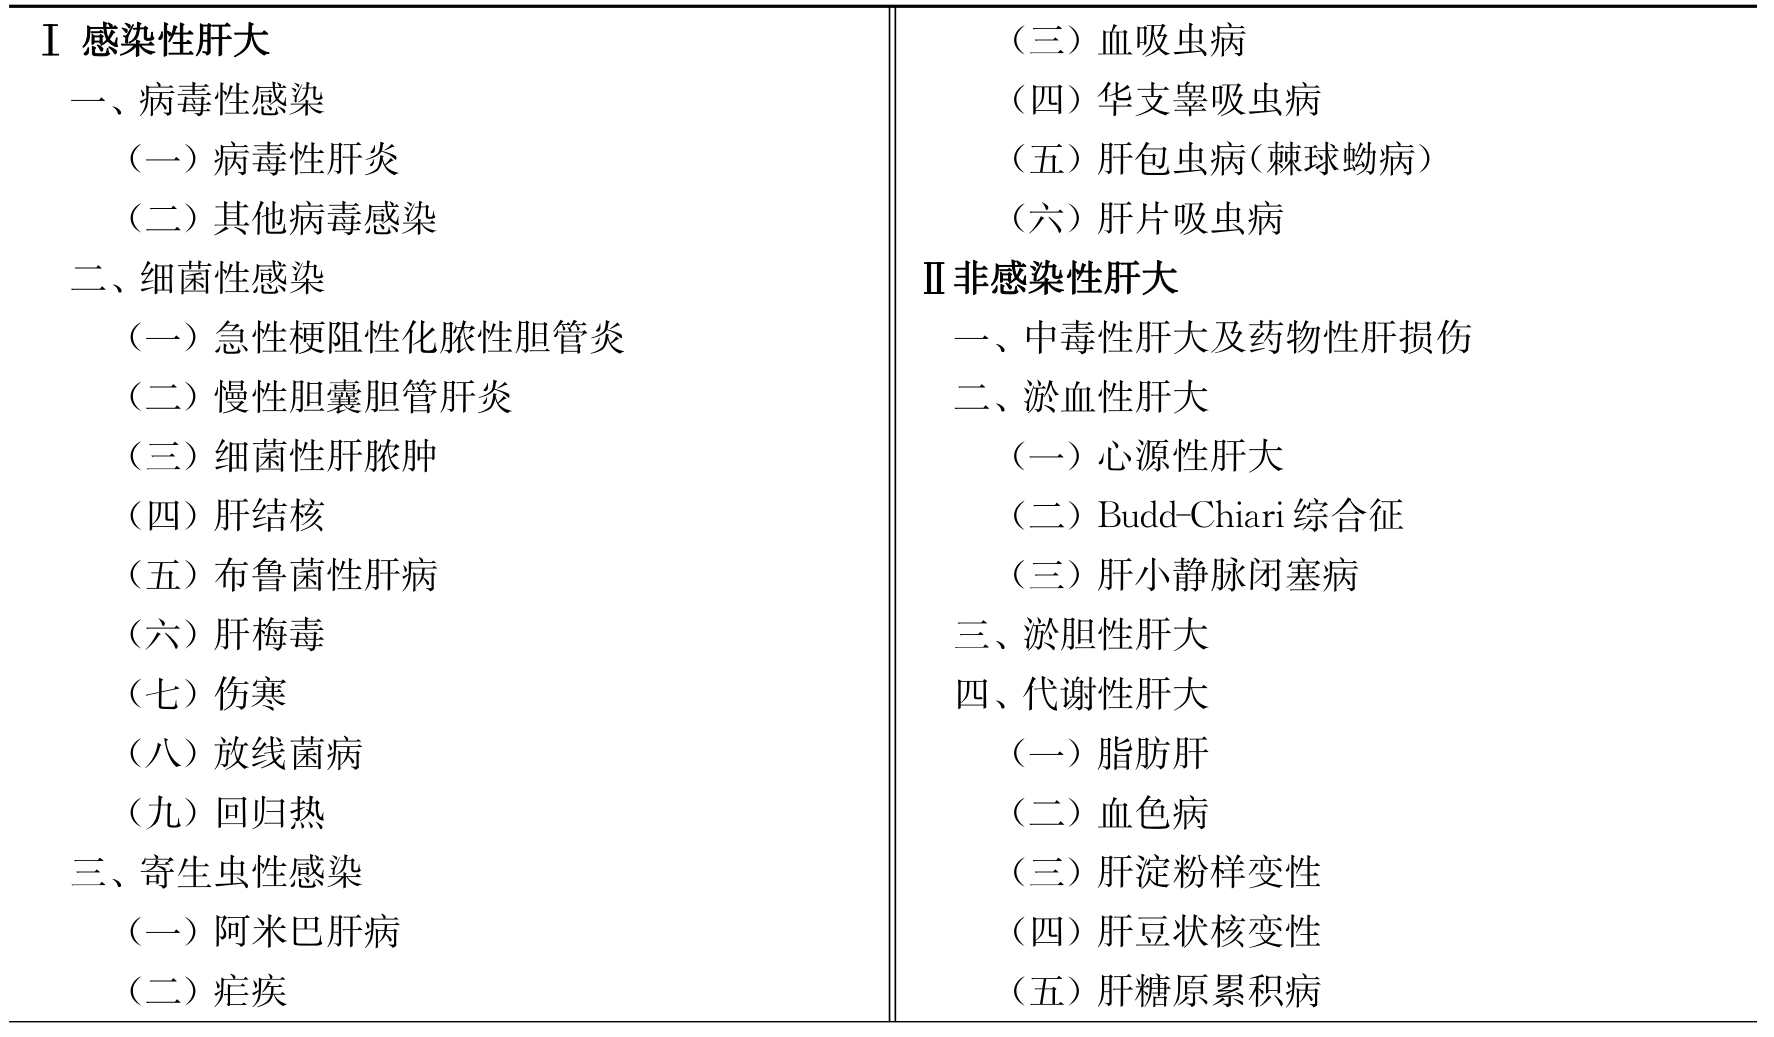
\includegraphics[width=\textwidth,height=\textheight,keepaspectratio]{./images/Image00156.jpg}\\
 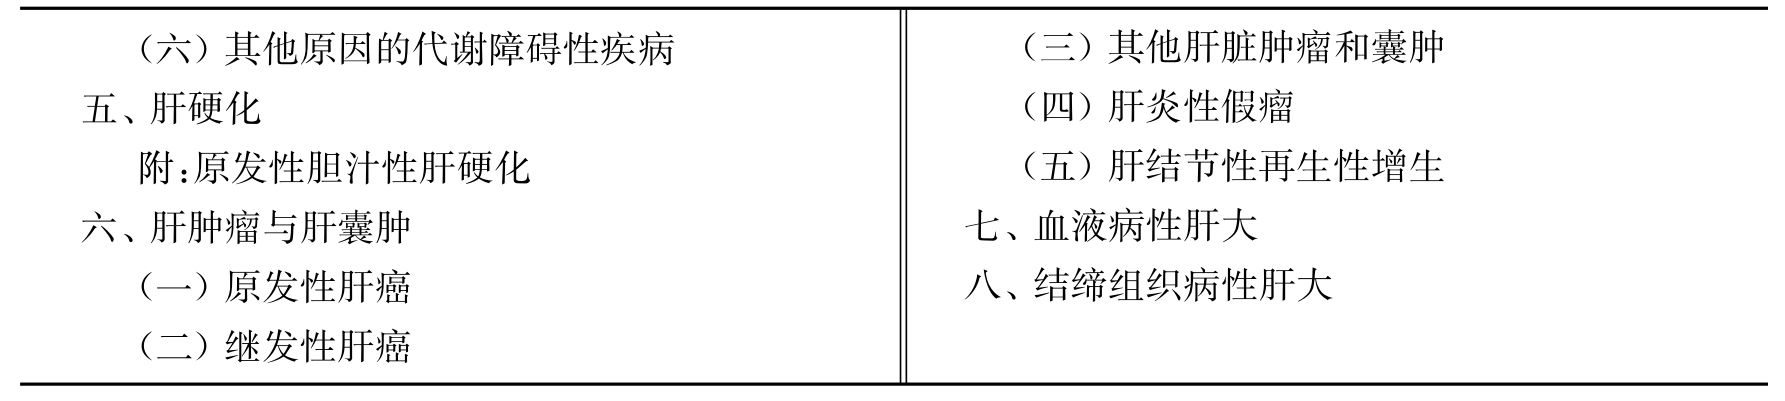
\includegraphics[width=\textwidth,height=\textheight,keepaspectratio]{./images/Image00157.jpg}
 \end{longtable}

\protect\hypertarget{text00239.html}{}{}

\section{106 感染性肝大}

\subsection{106.1 病毒性感染}

病毒性肝炎的临床分型及临床诊断依据已在第27章讨论。临床诊断必须有肝炎病毒学检测结果的证实,并做出病原学诊断。我国2000年制定的病毒性肝炎防治方案中,关于病原学诊断的标准有:

\subsubsection{(一)病原学分型}

目前病毒性肝炎的病原至少有五型,即甲型肝炎病毒(HAV)、乙型肝炎病毒(HBV)、丙型肝炎病毒(HCV)、丁型肝炎病毒(HDV)及戊型肝炎病毒(HEV)。

关于GBV-C/HGV和TTV的致病性问题尚有争议,且目前国内外尚无正式批准的诊断试剂可供检测,因此,不宜将GBV-C/HGV和TTV纳入常规病毒性肝炎的实验室检测。

\subsubsection{(二)各型病毒性肝炎病原学诊断依据}

\paragraph{1.甲型肝炎}

急性肝炎患者血清抗-HAV
IgM阳性,可确诊为HAV近期感染。在慢性乙型肝炎或自身免疫性肝病患者血清中检测抗-HAV
IgM阳性时,判断HAV重叠感染应慎重,须排除类风湿因子(RF)及其他原因引起的假阳性。接种甲型肝炎疫苗后2~3周约8\%~20\%接种者可产生抗-HAV
IgM,应注意鉴别。

\paragraph{2.乙型肝炎}

有以下任何一项阳性,可诊断为现症HBV感染:①血清HBsAg阳性;②血清HBV
DNA阳性;③血清抗-HBc IgM阳性;④肝内HBcAg和(或)HBsAg阳性,或HBV
DNA阳性。

\subparagraph{(1)急性乙型肝炎诊断:}

必须与慢性乙型肝炎急性发作鉴别。诊断急性乙型肝炎可参考下列动态指标:①HBsAg滴度由高到低,HBsAg消失后抗-HBs阳转;②急性期抗-HBc
IgM滴度高,抗-HBc IgG阴性或低水平。

\subparagraph{(2)慢性乙型肝炎诊断:}

临床符合慢性肝炎,并有一种以上现症HBV感染标志阳性。

\subparagraph{(3)慢性HBsAg携带者诊断:}

无任何临床症状和体征,肝功能正常,HBsAg持续阳性6个月以上者。

\paragraph{3.丙型肝炎}

\subparagraph{(1)急性丙型肝炎诊断:}

临床符合急性肝炎,血清或肝内HCV
RNA阳性;或抗-HCV阳性,但无其他型肝炎病毒的急性感染标志。

\subparagraph{(2)慢性丙型肝炎诊断:}

临床符合慢性肝炎,除外其他型肝炎,血清抗-HCV阳性,或血清和(或)肝内HCV
RNA阳性。

\paragraph{4.丁型肝炎}

\paragraph{(1)急性丁型肝炎的诊断:}

\subparagraph{1)急性HDV、HBV同时感染:}

急性肝炎患者,除急性HBV感染标志阳性外,血清抗-HDV IgM阳性,抗-HDV
IgG低滴度阳性;或血清和(或)肝内HDVAg及HDV RNA阳性。

\subparagraph{2)HDV、HBV重叠感染:}

慢性乙型肝炎患者或慢性HBsAg携带者,血清HDV
RNA和(或)HDVAg阳性,或抗-HDV IgM和抗-HDV IgG阳性,肝内HDV
RNA和(或)肝内HDVAg阳性。

\paragraph{(2)慢性丁型肝炎诊断:}

临床符合慢性肝炎,血清抗-HDV IgG持续高滴度,HDV RNA持续阳性,肝内HDV
RNA和(或)HDVAg阳性。

\paragraph{5.戊型肝炎}

急性肝炎患者血清抗-HEV阳转或滴度由低到高,或抗-HEV阳性>1∶20,或斑点杂交法或逆转录聚合酶链反应法(RT-PCR)检测血清和(或)粪便HEV
RNA阳性。目前抗-HEV IgM的检测试剂尚未标准化,仍需继续研究,但抗-HEV
IgM检测可作为急性戊型肝炎诊断的参考。

\subsubsection{(三)确立诊断}

凡临床诊断为急性、慢性、重型、淤胆型肝炎或肝炎肝硬化病例,经病原学或血清学特异方法确定为某一型的肝炎时即可确诊。两种或两种以上肝炎病毒同时感染者称为同时感染(co-infection)。在已有一种肝炎病毒感染基础上,又感染另一型肝炎病毒称为重叠感染(super-infection)。

确诊的肝炎病例命名是以临床分型与病原学分型相结合,肝组织病理学检查结果附后。例如:

(1)病毒性肝炎,甲型(或甲型和乙型同时感染),急性黄疸型(或急性无黄疸型)。

(2)病毒性肝炎,乙型(或乙型和丁型重叠感染),慢性(中度),G2S3(炎症活动程度2;纤维化程度3)。

(3)病毒性肝炎,丙型,亚急性重型,腹水型,早期(或中期或晚期)。

(4)HBsAg携带者近期感染另一型肝炎病毒时可命名如下:①病毒性肝炎,甲型(或戊型),急性黄疸型;②HBsAg携带者。

对甲、乙、丙、丁、戊五型肝炎病毒标志均阴性者可诊断为:急性肝炎,病原未定;或慢性肝炎,病原未定。

其他多种病毒性感染(如传染性单核细胞增多症、巨细胞病毒感染等)均可引起肝细胞损害而表现为肝大、转氨酶升高,但多有该病自身临床特征及实验室检查的变化,可资鉴别。

\protect\hypertarget{text00240.html}{}{}

\subsection{106.2 细菌性感染}

\subsubsection{一、急性梗阻性化脓性胆管炎}

急性梗阻性化脓性胆管炎可因肝充血与胆汁淤积而致肝大。本病以寒战(或恶寒)与发热、右上腹痛、胆汁淤积性黄疸为主征(参见第91.1节)。

\subsubsection{二、慢性胆囊胆管肝炎}

国内文献报道曾有从慢性无黄疸型肝炎病例中查出此病多例。其主要症状是右季肋部隐痛、食欲不振、厌油腻、恶心、腹胀、腹泻、消瘦等。微热也常见。肝轻度或中等度肿大,质多较硬,并有轻压痛。胆囊区压痛常存在。常规肝功能试验多属正常。十二指肠引流胆汁细胞数每高倍镜视野往往20个以上,半数以上培养阳性,最多为大肠杆菌。多次的十二指肠引流阳性结果,有助于此病的诊断。部分病例胆囊造影不正常,有些经手术证明为慢性胆囊炎或兼有胆石症。

目前,对这些病例的诊断尚存在疑问,该病名亦未为多数学者所认同。

\subsubsection{三、细菌性肝脓肿}

细菌性肝脓肿常以恶寒或寒战、高热、右上腹疼痛、肝大与压痛为主要症状起病。疼痛可向右肩放射(右叶脓肿)。有时出现黄疸。白细胞常明显增多与中性核左移。提示细菌性肝脓肿的诊断是,在腹腔化脓性感染或败血症病程中出现肝大与疼痛。如患者急性阑尾炎或其他腹腔化脓性疾病手术之后,突然出现上述症状,应考虑此病的可能性。国内报告隐源性者有达40.5\%之多。

细菌性肝脓肿尚可区分为单发性与多发性两种,但临床上难准确判别。通常可根据临床表现以初步鉴定之。多发性细菌性肝脓肿发病通常急骤,病程短,且高热、寒战、恶心、呕吐等症状皆较严重,肝两叶同时肿大,多有脾大,白细胞增多较显著,原发病如化脓性阑尾炎、化脓性胆管炎、败血症等较易查出。原发病灶不明与起病缓慢者以单发性脓肿为多见。有局限性隆起者也支持单发性肝脓肿。肝大为常见体征,达60\%~90\%,肝区压痛或叩击痛更常见。病变浅在者可有局限性腹膜刺激症状。小而深的脓肿可无任何体征。

细菌性肝脓肿的病原菌主要为大肠杆菌与金黄色葡萄球菌,少数为铜绿假单胞菌、变形杆菌等。伤寒杆菌性肝脓肿罕见,通常为单发性,位于右叶。

应用B超诊断肝脓肿,对其部位、数量、大小都能较明确的提示。但是,超声诊断肝脓肿也有时误诊,主要是将已有液化的肝内肿瘤误诊为肝脓肿,也有将肝脓肿误诊肝癌等者,密切的临床动态观察可减少误诊率。过去常将肝脓肿误诊为急性胆囊炎,自超声检查广泛应用以来已大为减少。胆囊炎常有各种原因的胆道梗阻为发病基础,胆囊区压痛与肌紧张较明显,且有胆囊触痛征。CT检查也有重要诊断价值。

细菌性肝脓肿须与阿米巴肝脓肿相区别,后者40\%~50\%患者有肠阿米巴病或腹泻病史,起病较慢,常无高热与明显的白细胞增多,肝大常较明显,脓液呈巧克力样(棕褐色)色,有时可找到溶组织阿米巴滋养体,脓液常较细菌性肝脓肿多,一次穿刺抽得100ml以上者多见,抗阿米巴治疗有效。

由于胆总管结石或胆道蛔虫梗阻所致的肝脓肿,通常为两叶多发性,这是由于胆道系统感染后,细菌(通常为大肠杆菌)沿肝内小胆管播散所致,同时被堵塞的肝内胆管有明显的扩张或憩室形成,并于局部形成脓肿,故也称为“胆管性肝脓肿”。

细菌性肝脓肿又须与右膈下脓肿相区别。膈下脓肿同样也发生于腹部手术后或腹部化脓性感染之后。在上述情况时患者仍有脓毒血症症状存在,而未发现化脓性病灶,且触诊右肋缘或右背部沿第12肋骨有压痛,听诊右肺底呼吸音减弱或消失,提示此病的诊断线索。X线透视发现横膈上升与固定、膈下有气泡与液平面,即可确定诊断。超声也可有助于与肝脓肿相鉴别,并有助于穿刺的定位。B超引导下定位穿刺排脓对肝脓肿的诊断和治疗有重要价值,必要时可置管引流。脓液细菌培养可指导抗生素的使用。

\subsubsection{四、肝结核}

患者有原因未明的肝大,尤其是青壮年人,合并发热、食欲不振、乏力、消瘦、盗汗等结核中毒症状,应警惕肝结核的可能性。如同时有体内其他脏器的结核病灶,则可能性更大。发病大多在青壮年,发热特点是多呈弛张型热,不伴发冷而多有盗汗。肝大多伴自觉痛与触痛。血沉加快。中等度贫血。白细胞计数多属正常或减少。半数有肝功能损害,为胆红素增高、白蛋白降低和球蛋白升高、ALP增高及染料排泄试验异常。

肝结核不是一个独立的疾病,常系全身性结核播散的一部分。也有些病例,临床上主要表现为肝脏病病征,而缺乏体内其他结核病灶的病征,且有些肝脏病的临床表现已很明显,并经肝活检证明为肝粟粒型结核,但X线肺部检查仍为阴性。因此,临床上一般对以肝脏病表现为主的肝内结核,同时伴有不大明显或隐伏的体内其他结核病灶,均称之为“原发性”肝结核。

由于肝结核无特异性病征,临床上难以作出诊断,每易误诊为伤寒、慢性黄疸型或无黄疸型肝炎、肝硬化、肝脓肿、慢性胆囊炎甚或肝癌与恶性淋巴瘤。多数病例需要肝穿刺活检才能明确诊断。有认为青年人未明原因的发热,伴肝或上腹胀痛、肝大伴触痛、食欲减退、中度贫血、白细胞数减少或正常、血沉加快、肝功能损害,提示本病的诊断。结核菌素试验多呈阳性,有结核瘤或脓肿者,B超、CT或MRI可发现占位性病变。腹腔镜检查诊断肝结核安全而可靠,在直视下作粟粒结节活检,效果远胜于盲目的肝穿刺。可作抗结核治疗。

\subsubsection{五、布鲁菌性肝病}

布鲁菌性肝病临床上可表现为急性肝炎、慢性肝炎与肝硬化三型。急性肝炎型类似急性无黄疸型病毒性肝炎,有发热、食欲减退、厌油、腹胀、恶心、呕吐、肝大与压痛、血清絮状与浊度反应阳性等表现,但患者有相应的波状热流行病史,发热较高较长,有关节痛、多汗等症状,血清布鲁菌凝集反应阳性、血培养可证明布鲁菌,均有助于两者的鉴别。

慢性肝炎型常有间歇的微热,病程迁延,主要表现为原因未明的肝、脾大,如同时伴有关节炎及睾丸炎,则有助于与慢性无黄疸型病毒性肝炎相鉴别。慢性肝炎型布鲁菌病时,血及骨髓培养阳性率较低,血清布鲁菌凝集滴度可较低甚至阴性。故上述检查阴性结果未能除外此病,有怀疑时宜进一步作组织培养。

肝硬化型可出现门静脉高压症状与显著脾大,如病原学与血清学检查未能证实此病,可考虑肝穿刺活检以确定之,一般发现布鲁菌性肉芽肿的机会较高。

\subsubsection{六、肝梅毒}

肝梅毒临床上罕见,国内仅有少数病例报告,均系在解放前感染者。成年人梅毒都为后天性,常发生于感染后的第二期与第三期,因此有早期梅毒与后期梅毒之分。

早期肝梅毒的特点是弥漫性肝炎,多有黄疸、肝大的症状,临床上可与散发性病毒性肝炎相混淆。其不同点为患者有梅毒接触史或感染史,缺乏明显的胃肠道症状,而有其他二期梅毒病征,血沉加快,血清梅毒反应常为阳性。驱梅治疗有佳良效应,也有助于诊断。

后期肝梅毒的特点是树胶肿形成。树胶肿痊愈时形成瘢痕组织,引起肝脏变形,在肝表面形成深沟,将肝脏分为多个大小不等的部分------此即所谓分叶肝。肝大而表面凹凸不平,质硬,一般无压痛。驱梅疗程往往显著缩小。患者全身情况佳良,梅毒血清反应阳性率高达90\%,甚有助于诊断。鉴别诊断上须注意者为肝癌,因也可有不规则的肝大。肝癌为进行性恶性变,当有明显肝大时全身情况较差,甲胎蛋白放射免疫测定、梅毒血清反应等检查,均有助于与肝梅毒鉴别。

\subsubsection{七、伤 寒}

伤寒是由伤寒杆菌经消化道侵入而引起的急性传染病。典型病例以持续发热、全身中毒症状、相对缓脉、玫瑰疹、脾大与白细胞减少等为特征。30\%~40\%有肝大,多为轻至中度肿大,重者可有黄疸。实验室检查:病程中白细胞数减少,分类中淋巴细胞相对增加,嗜酸性粒细胞减少或消失。血培养、骨髓培养等发现病原体。血培养早期可阳性,第七至九日时阳性率可达90\%。骨髓培养阳性率较血培养高,尤适用于已用抗生素治疗但血培养阴性者。肥达反应中“0”效价≥1∶80和“H”效价≥1∶160者,可以诊断为伤寒。一般在第二周阳性率增高。

\subsubsection{八、肝放线菌病}

本病系肠道放线菌病的后果,尤其是阑尾和盲肠放线菌病。放线菌可直接扩散,或经门静脉散布至肝脏。多需病理活检或术后病理检查才能诊断。病变呈灰白色肿块,液化后形成脓肿,被纤维隔所分开,呈蜂窝状。脓液中可检出放线菌菌落,脓肿周围可见大量巨噬细胞、淋巴细胞。

\subsubsection{九、回归热}

回归热是回归热螺旋体引起的急性传染病。其临床特点是急起急退的发热,伴全身酸痛、肝脾大,重症有黄疸和出血倾向。继无热间歇期后,又可出现周期性一次或多次的反复发作。临床表现:潜伏期平均约一周(虱传型2~14天,蜱传型4~9天)。有时可有头昏、乏力、低热等l~2天的前驱症状。绝大多数起病急骤,畏寒、寒战,继以高热,剧烈头痛和全身肌肉骨骼疼痛为突出症状,以腓肠肌明显。2/3肝大伴压痛,3/4脾脏明显肿大。部分患者有恶心、呕吐等。体温在1~2天可达40℃左右,大多呈持续型,少数为弛张型或间歇型。发热持续6~7天后体温骤降,伴以大汗,甚至出现休克症状。在无热间歇期间,患者除感虚弱无力外,其他症状减退或消失,肝脾大及黄疸等也随之消失。经过平均7~9天的间歇期后,多数患者再度出现全身症状,复发后往往症状较轻,病程也较短。以后间歇期逐渐延长。诊断:有典型的临床表现,如急起发热,伴剧烈头痛、全身肌肉和关节酸痛、肝脾大、皮疹及黄疸等,结合当地流行情况、季节、个人卫生或野外作业史作出初步诊断。当发热呈回归型并有多次复发者则诊断可基本成立。从周围血液或重症患者的尿、脑脊液中发现螺旋体或接种小白鼠阳性均可确立诊断。血清特异性抗体增高4倍以上也有助于诊断。

\protect\hypertarget{text00241.html}{}{}

\subsection{106.3 寄生虫性感染}

\subsubsection{一、阿米巴肝病}

阿米巴肝炎与阿米巴肝脓肿合称为阿米巴肝病。此病是肠阿米巴病的重要并发症。

阿米巴肝病的早期表现是阿米巴肝炎。阿米巴肝炎无特征性症状,通常表现为原因未明的持续发热,其特点是缓慢起病而无寒战,一般为中等度弛张热,肝轻度乃至中等度肿大并有压痛。血象白细胞常轻度或中等度增多(一般不超过15
000/mm\textsuperscript{3}
),分类计数中性粒细胞85\%~90\%,合并轻度左移。黄疸少见,有之亦为轻度。如患者有痢疾病史或证实曾患肠阿米巴病,尤值得怀疑。如已排除其他原因(特别是败血症)的感染性肝大,应进行甲硝唑诊断性治疗,以免酿成肝脓肿。

如已形成肝脓肿,全身症状较为明显,肝区痛较剧,常向肩部放射,局限性压痛也较显著。局限性压痛通常位于右侧腋前线与腋中线之间的第7、8肋间,对提示诊断有意义,在未有超声波诊断之时,诊断性穿刺部位通常在压痛点进行。80\%的脓肿位于右叶,如位于顶部,X线透视可发现右膈局限性隆起;如位于左叶,钡餐透视可发现胃压迹与移位。超声诊断肝脓肿有重要价值,可显示脓肿的大小与部位,对诊断性与治疗性穿刺(左叶脓肿时须慎重)有帮助。阿米巴肝脓肿的特征性表现是脓液呈棕褐色,镜检可发现溶组织阿米巴滋养体,但阳性率不高。形成肝脓肿后肝脏肿大更加显著,下界可平脐,压痛明显。

国内报告在阿米巴肝病患者作反复的十二指肠引流,约2/3病例可在胆汁(尤以丙胆汁)中检出阿米巴滋养体。此法对阿米巴肝病有早期诊断价值,尤以高度怀疑此病而超声检查阴性时。

阿米巴肝病是容易误诊与漏诊的肝脏疾病之一。此病在国内分布甚广,尤以华南、华东一带比较多见。误诊的原因大多由于对此病注意不够,同时也可能由于此病的表现多样化。有些病例可能由于病变在肝内进展缓慢,或曾接受不规则的抗生素(四环素族、红霉素)治疗,致病情稍受抑制,肝脓肿呈慢性经过,此时患者全身情况较差、发热、消瘦、肝大而硬、压痛可不明显,易被误诊为肝癌。另一方面,晚期肝癌的中心部液化,超声表现与肝脓肿相似,也应注意。诊断性抗阿米巴治疗以及血清甲胎蛋白测定常有助于两者的鉴别。如无禁忌证(如出血倾向等),在超声定位下小心进行诊断性穿刺,对两者鉴别有重要帮助。

阿米巴肝病的血清学诊断,目前认为以间接血凝试验(IHA)检测阿米巴抗原较有价值,特异性高,高滴定度(1∶128以上)常见于阿米巴感染。阿米巴肝脓肿脓液中仅20\%~50\%病例可检出阿米巴滋养体,可采取脓液沉淀的上清液作阿米巴抗原检查,阳性结果对诊断有较大的帮助。

少数阿米巴性肝脓肿合并细菌感染,大多为大肠杆菌,脓液有粪臭味。

\subsubsection{二、疟 疾}

疟疾是疟原虫经蚊传播而引起的寄生虫病。疟原虫经血液侵入肝细胞和红细胞内寄生繁殖,使红细胞成批破裂而发病。其临床特点为间歇性定时发作的寒战、高热,继以大汗而缓解。多次发作后脾脏明显肿大,伴贫血。半数以上伴有肝大,多为轻度肿大,约1/3病例有压痛。临床表现:潜伏期:间日疟潜伏期短者为13~15天,长者达6个月以上;三日疟约为24~30天;恶性疟为7~12天;卵形疟为13~15天。部分患者有前驱症状,如疲倦、乏力、头痛、肌肉酸痛、食欲减低等。典型的发作为周期性寒热发作,隔日一次或3天一次。发热时有明显的寒战、高热和大汗,伴头痛、肌肉酸痛、乏力、恶心呕吐。继以症状明显缓解。恶性疟者可出现凶险发作如脑型疟疾,表现为急起高热,剧烈头痛、呕吐、谵妄。血片中易查见疟原虫。严重者可发生脑水肿、呼吸衰竭而死亡。过高热型表现为持续高热,可达42℃,谵妄,继以昏迷、抽搐,可于数小时内死亡。

诊断:①流行病学资料:有在疟疾流行地区居住或旅行史,近年有疟疾发作史或近期接受过输血。②有典型的临床表现。③血象中白细胞正常或减少,分类中大单核细胞增多。寒战发作时取血涂片染色查疟原虫,或做厚血片检查及骨髓穿刺涂片检查疟原虫。血中或骨髓查到疟原虫是确诊的最可靠依据。④亦可用氯喹(3天)作诊断性治疗。治疗后体温下降,症状消失不再出现者可拟为疟疾。

\subsubsection{三、血吸虫病}

急性血吸虫病约80\%有肝大。肝大的程度与病情相平行,其出现也早,至病程的4~5周达高峰,重症者肝下缘可达脐下,叩击痛与压痛都很明显。特别是剑突下的压痛是本病的重要体征。重症病例肝区可有剧痛,放射至肩部,右上腹壁紧张,每被误诊为肝脓肿。肝功能改变主要表现为间质反应,而肝实质损害较轻(清蛋白与球蛋白比值的异常百分率随肝大程度而增加,但转氨酶升高程度较轻,大多在200U以下)。其他的表现包括发热、腹痛、腹泻及咳嗽、胸痛、气喘等呼吸道症状。

轻症慢性血吸虫患者多无自觉症状,或有轻度消化不良症状,体检常可发现轻度肝、脾大。血吸虫尾蚴接触史提供重要的诊断线索。血吸虫抗原皮内试验与超声检查也有辅助诊断意义。直肠镜活检血吸虫卵阳性率相当高,对此病诊断有重要意义。

重症病例晚期发展为肝硬化,肝脏此时多已缩小,但部分病例仍可触及,表面呈结节状,硬度明显增加。可出现脾大、腹水、食管胃底静脉曲张、下肢水肿等肝硬化失代偿期的表现。此时诊断应追溯既往病史,血吸虫抗原皮内试验也有辅助诊断价值。有人发现晚期病例直肠黏膜活检仍易找到虫卵。

\subsubsection{四、华支睾吸虫病}

华支睾吸虫寄生于肝内胆管中,对肝实质损害较轻。轻症华支睾吸虫感染无肝大,也无自觉症状,但重症感染则常有轻度或中等度肝大。国内一组病例报告有肝大者为59.9\%,且多伴有压痛。患者多诉倦怠无力,或尚有食欲减退、上腹饱胀、腹痛、腹泻、恶心、呕吐等症状。吃生的或未熟透的鱼(受感染的鱼)史提供此病的诊断线索。超声检查有比较特别的波形,肝内胆管可有扩张,有一定的辅助诊断价值。粪便和胆汁虫卵检查可确定诊断。集卵法较易从大便中发现虫卵。逆行胆管造影可显示胆总管扩张及成虫在胆管聚积形成的充盈缺损。

由于上述的症状和部分病例血清谷-丙转氨酶活性升高,此病易误诊为病毒性肝炎。此病时,谷-丙转氨酶活性升高通常在300U以下,全身症状与消化系症状一般也较肝炎轻,且各有不同的流行病学史,肝炎病毒标志物检测有助于两者的鉴别。

特别是急性华支睾吸虫病,症状酷似急性病毒性肝炎,诊断主要依据病史与华支睾吸虫抗原皮试。

另一方面,华支睾吸虫病常为肝胆道感染和胆石症的发病基础,并由此导致胆囊炎、胆石症或胆管炎性肝炎,反复的十二指肠胆汁引流有助于诊断。血中嗜酸性粒细胞增多,ELISA可检查血清特异性抗体或血清循环抗原。

\subsubsection{五、肝包虫病(棘球蚴病)}

包虫病多见于牧区,最多发生于肝脏。肝大为肝包虫病必有的体征,最多位于右叶,通常为单房性(囊型肝包虫病)。早期往往有类似胆囊炎的症状,心窝部有胀满感,进食后上腹部不适,恶心,有牵引性钝痛,或伴有肩部放射痛。囊肿位于右叶顶部时,X线透视下右膈肌呈半圆形隆起;囊肿位于肝脏中心时,常引起肝脏普遍性肿大;囊肿靠近肝下缘时,往往可触及肋缘下一个半圆形突出的、表面平滑的硬块,随呼吸而上下移动,指压之呈硬韧而富有弹性的囊样感;在巨大的单房性囊肿可试出包虫囊震颤感。囊肿压迫胆总管时引起阻塞性黄疸;压迫门静脉时可引起腹水。

多房性肝包虫病也称泡型肝包虫病,是肝包虫病的一种异型,肝呈软骨样硬度,表面凹凸不平,酷似肝癌、肝硬化或肝梅毒,超声检查表现多样性与复杂性、类似肝癌的波型,须结合全面检查材料鉴别之。

肝包虫病的诊断主要根据:

1.患者有与犬密切接触史,肝大(尤其是局限性者)而肝脏病症状不明显,血中嗜酸性粒细胞增多。

2.X线检查右膈变形或蛋壳样钙化的囊壁;超声检查肝内含充满液体的囊腔。

3.皮内抗原试验(Casoni法):取0.2ml
1∶4~100倍稀释的无菌包虫抗原液注入患者皮内,阳性反应时出现一个潮红硬结、直径23mm以上,典型者呈蟹足状红斑。单纯性包虫病阳性率75\%左右,有囊肿破裂等合并症后,初期阳性率高达95\%,但在某些变态反应疾病和蠕虫病也可呈假阳性。阴性反应约95\%可除外包虫病。

4.血清补体结合试验:约70\%~80\%患者(有活包虫寄生的)血清中可证明特异性补体结合抗体。

近年日本学者通过简单的酚/氯仿法从粗制的泡球蚴提取物中分离出一种C抗原,对诊断泡型肝包虫病的敏感性和特异性,分别为95\%与100\%。

肝顶部包虫囊肿有时与位于肺底者甚难鉴别,下列X线征象可供参考:①肺包虫囊肿与胸腔内壁之间可有空隙,肋膈角常存在,而肝顶部囊肿间膈肌突出,并占满胸腔下部,与胸腔内壁之间的空隙和肋膈角均消失。②肝顶部包虫囊肿常使心脏移位,而肺底部囊肿仅在较大之时才使心脏轻度移位。③肺包虫囊肿与膈肌所形成的角度多为锐角,而在肝顶部囊肿多为钝角。必要时可采用人工气腹以鉴别之。

\subsubsection{六、肝片吸虫病}

肝片吸虫病主要在家畜中传播,以羊为主要终宿主,人饮用被囊蚴污染的生水或食用被囊蚴污染的水生植物而感染。国内有局部流行的存在。

本病急性期以发热、腹痛、进行性肝大与贫血、肝功能损害、嗜酸性粒细胞增多、高球蛋白血症为主要表现。慢性期表现为右上腹疼痛、恶心、纳差、肝大、阻塞性黄疸等,易被误诊。诊断须根据流行病学史、粪便或十二指肠引流中找到肝片吸虫卵。

\protect\hypertarget{text00242.html}{}{}

\section{107 非感染性肝大}

\subsection{107.1 中毒性肝大及药物性肝损伤}

药物和化学制剂进入人体引起的肝损害,常导致肝大和黄疸。近年来,药物性肝病的发病率在逐渐增高,临床表现可多样化,从仅有轻度肝功能损害到暴发性肝衰竭均可出现。中毒性肝炎一般有肝毒物质的直接接触史,病变严重程度与剂量有直接关系,所有接触者均可致病。药物过敏性肝损害由药物过敏所致,某些药物可造成胆汁分泌功能障碍而引起黄疸,长期过量用药所致的肝损害可能是过多的药物增加了肝脏代谢负担。这类疾病的特点是:①中毒性肝炎潜伏期较短,而药物性肝炎则长短不一。②临床表现与病毒性肝炎类似,有黄疸、肝大并有压痛,有时脾大。伴有恶心、呕吐、纳差、乏力、尿黄等。严重者可有亚急性肝坏死等。停药后大都于短期内恢复,少数患者可形成肝硬化。③中毒性肝炎无黄疸前期的发热及周身症状,而药物性肝炎常迅速出现过敏反应性周身症状,如发热、腹泻、皮疹、瘙痒、关节痛等,并常伴以纳差、恶心、呕吐、腹痛等。黄疸往往与其他过敏症状相继出现,严重者有白细胞减少、血小板减少、血管神经性水肿、剥脱性皮炎等。

药物性肝损伤诊断标准:①有与药物性肝损伤发病规律相一致的潜伏期:初次用药后出现肝损伤的潜伏期一般在5~90天内,有特异质反应者潜伏期可<5天,慢代谢药物(如胺碘酮)导致肝损伤的潜伏期可>90天。停药后出现肝细胞损伤的潜伏期≤15天,出现胆汁淤积性肝损伤的潜伏期≤30天。②有停药后异常肝脏指标迅速恢复的临床过程:肝细胞损伤型的血清ALT峰值水平在8天内下降>50\%(高度提示),或30天内下降≥50\%(提示);胆汁淤积型的血清ALP或TB峰值水平在180天内下降≥50\%。③必须排除其他病因或疾病所致的肝损伤。④再次用药反应阳性:有再次用药后肝损伤复发史,肝酶活性水平升高至少大于正常值上限的2倍。符合以上诊断标准的①+②+③,或前3项中有2项符合,加上第④项,均可确诊为药物性肝损伤。

\subsection{107.2 淤血性肝大}

\subsubsection{一、心源性肝大}

淤血性肝大是心包炎或右心衰竭的重要病征。急性心包炎时,表现有心前区疼痛,心包填塞症状和全身症状。心包积液迅速发生时,表现为心动过速,心浊音界扩大、心音遥远、奇脉,心排出量明显下降,可导致休克。缓慢发生的心包积液或缩窄性心包炎,除心率加快外,可见静脉压显著升高,肝大伴触痛、腹水、颈静脉怒张、皮下水肿、肝颈静脉反流征阳性等循环淤血表现,收缩压下降、脉压减少、脉搏细弱、出现奇脉。肝大和压痛系右心衰竭早期表现,多发生于皮下水肿之前。肝大以剑突下为明显,肝区疼痛且有触痛。右心衰竭突然加重时,肝脏急剧肿大,随心力衰竭好转而缩小。长期慢性右心衰竭引起心源性肝硬化时,肝脏触诊质地较硬,压痛不明显,常伴黄疸、腹水及慢性肝功能损害。

\subsubsection{二、Budd-Chiari综合征}

本病是指肝静脉流出道阻塞所引起的以肝脏排血障碍为主要表现的综合征。临床表现和阻塞部位、程度及起病缓急有关。常分为急性、亚急性和慢性三种。以慢性型最常见,易和肝硬化混淆,但一般无病毒性肝炎病史。患者肝窦扩张淤血,肝脏肿痛,大量腹水,肝尾叶增大为其特征。该病的诊断参见第92节。

\subsubsection{三、肝小静脉闭塞病}

本病少见,可引起肝大与腹水,病征与Budd-Chiari综合征相似,应注意鉴别,参见第92节。

\subsection{107.3 淤胆性肝大}

多种病因引起的胆汁淤积均可引起不同程度的肝大,病程长者可发展为胆汁性肝硬化。发生胆汁淤积的疾病详见第91节。

\subsection{107.4 代谢性肝大}

\subsubsection{一、脂肪肝}

脂肪肝是由多种疾病和病因引起的肝脏脂肪性变。患者常有慢性长期饮酒史,或因蛋白质、热量摄入不足而营养不良,或有肥胖症、糖尿病史。随着我国居民饮食结构的变化及乙醇消耗量的增加,脂肪肝的发病率在上升。脂肪肝一般分为乙醇性脂肪肝和非乙醇性脂肪肝。乙醇性脂肪肝是乙醇性肝病中的一个类型。在乙醇性肝病的组织学改变,乙醇性脂肪肝出现最早,出现率也最高,但临床症状并不明显,可有轻微肝区不适、隐痛、肝大、纳差等。酒精性肝病诊断标准:①有长期饮酒史,一般超过5年,折合乙醇量男性≥40g/d,女性≥20g/d,或2周内有大量饮酒史,折合乙醇量>80g/d。但应注意性别、遗传易感性等因素的影响。乙醇量(g)=饮酒量(ml)×乙醇含量(\%)×0.8。②临床症状为非特异性,可无症状,或有右上腹胀痛、食欲不振、乏力、体重减轻、黄疸等;随着病情加重,可有神经精神症状和蜘蛛痣、肝掌等表现。③血清AST、γ-谷氨酰转肽酶、TBil、Pr、平均红细胞容积(MCV)和缺糖转铁蛋白(CDT)等指标升高。其中AST/ALT>2、GGT升高、MCV升高为酒精性肝病的特点,而CDT测定虽然较特异但临床未常规开展。禁酒后这些指标可明显下降,通常4周内基本恢复正常(但GGT恢复较慢),有助于诊断。④肝脏超声检查或CT检查有典型表现。⑤排除嗜肝病毒现症感染以及药物、中毒性肝损伤和自身免疫性肝病等。符合第1~3项和第5项或第1、2、4项和第5项可诊断酒精性肝病;仅符合第1、2项和第5项可疑诊酒精性肝病。符合第1项,同时有病毒性肝炎现症感染证据者,可诊断为酒精性肝病伴病毒性肝炎。

非酒精性脂肪性肝病诊断标准:明确NAFLD的诊断需符合以下3项条件:①无饮酒史或饮酒折合乙醇量小于每周140g(女性<每周70g);②除外病毒性肝炎、药物性肝病、全胃肠外营养、肝豆状核变性、自身免疫性肝病等可导致脂肪肝的特定疾病;③肝活检组织学改变符合脂肪性肝病的病理学诊断标准。鉴于肝组织学诊断难以获得,NAFLD工作定义为:①肝脏影像学表现符合弥漫性脂肪肝的诊断标准且无其他原因可供解释;②有代谢综合征相关组分的患者出现不明原因的血清ALT和(或)AST、GGT持续增高半年以上。减肥和改善IR后,异常酶谱和影像学脂肪肝改善甚至恢复正常者可明确NAFLD的诊断。

\subsubsection{二、血色病(hemochromatosis)}

血色病又名古铜色糖尿病,是一种铁储存过多疾病,属常染色体隐性遗传。具有明显家族性。临床上罕见。典型病象有皮肤色素沉着、肝大、糖尿与性功能减退。肝轻度或中等度增大,表面平滑,中等硬度,可有轻压痛,发展为肝硬化时肝缩小而硬度明显增加。病程长,发病多在中年以后,但国内报告也有发生于青壮年。男性罹患远多于女性。皮肤灰棕色或古铜色色素沉着可遍及全身,但以颜面、颈项及前臂等暴露部位较明显,黏膜多不受累,此点与慢性肾上腺皮质功能减退症有别。

此病具有典型病象者不多,故甚易漏诊。如发现患者有皮肤色素沉着与硬度增加的肝大,应考虑此病的可能性。皮肤试验(Fishbach法)在本病时显示普鲁士蓝反应,有辅助诊断价值,但肝组织活检的诊断意义更大。可见含铁血黄素或黑色素沉积。

血清铁蛋白(ferritin)水平是反映体内铁储存量的指标,其血清中浓度与血色病病情相平行。血色病时血清铁蛋白可达到正常人的5~10倍,有重要诊断意义。血清铁及转铁蛋白饱和度也可显著增高。CT或MRI检查肝有过量铁沉积的改变。

血色病须与继发性含铁血黄素沉着症相区别:前者与机体铁代谢失常有关;后者常起于长期大量输血或长期大量应用铁剂之后。

血色病可发展为肝硬化,与门脉性肝硬化的临床表现相似。

\subsubsection{三、肝淀粉样变性}

肝淀粉样变性非常少见,可分为继发性与原发性两型,继发性者均为全身性,常可证明原发病的存在。国内仅有少数全身性淀粉样变伴有肝淀粉样变病例报告。临床上如患者有质硬、无压痛、表面光滑而边缘钝的肝大,同时伴有慢性化脓性感染(特别是慢性骨髓炎、慢性肺脓肿等)、结核病、类风湿关节炎等疾病时,应考虑此病的可能性。可有巨舌症,对提示原发性型的诊断有意义。黄疸一般不存在。肝功能损害极轻,甚至有广泛的肝淀粉样变性时也是如此。如有大量蛋白尿、血清胆固醇升高而血压正常,提示兼有肾淀粉样变性。还可累及心、胃肠道等,引起充血性心力衰竭、小肠吸收不良。阳性刚果红试验(90\%~100\%可被吸收)是诊断此病的重要检查方法,但阴性未能排除此病。如试验结果不满意,可考虑肝穿刺活检,活检标本也可采自牙龈、皮肤、肌肉等组织。近年来发现一些没有上述相伴疾病的原发性全身性(包括肝脏)淀粉样变性病例,其临床表现与上述形同,但脏器中的淀粉样物质对刚果红的亲和力可甚低,故刚果红试验不少呈阴性而需由活检来确诊。

伴有肝、脾大的淀粉样变性,须与门脉性肝硬化相区别,主要仍根据肝大的性质、较轻的肝功能损害、其他脏器的淀粉样变性、刚果红试验与病理组织活检。

\subsubsection{四、肝豆状核变性(Wilson病)}

此病发病与铜代谢失常有关,有明显家族史,属于常染色体隐性遗传,多见于儿童和青少年,一般起病缓慢,少数急性发病。多数病例有肝功能损害,并可发展为肝硬化,但临床上可有不同程度的表现。患者多以神经症状为主而就诊,如震颤、流涎、手足徐动、特殊步态等。较少以肝病为主要症状而就诊,少数患者就诊时神经症状可未出现,此时易被误诊为肝炎肝硬化。

目前公认,患者血清铜蓝蛋白浓度和血清铜氧化酶活性,均较正常人明显降低,因而是诊断肝豆状核变性最有用的指标,也是本病与原发性胆汁性肝硬化和慢性活动性肝炎相鉴别的主要生化学指标,因后两者血清铜蓝蛋白浓度和血清铜氧化酶活性均在正常范围。角膜可见色素环亦有助诊断。肝活检肝细胞有铜颗粒沉积。

\subsubsection{五、肝糖原累积病}

糖原累积病是一种罕见的先天性碳水化合物代谢失常疾病,主要侵犯肝、心肌、肾及肌肉等器官。此病通常发生于幼儿或儿童时期,主要临床表现是肝大、低血糖、高血脂与高胆固醇、酮尿、发育迟滞等。患儿常有软弱、乏力、厌食、体重减轻、腹胀、呕吐等症状。肝明显肿大,表面平滑,质较硬而无压痛。多数患儿不能存活至成年。葡萄糖耐量曲线上升后降落甚慢;胰高血糖素试验血糖升高反应不敏感(正常注入0.5mg后10~20分钟空腹血糖上升3~4mmol/
L,本病患者上升<0.1mmol/L),均为诊断此病比较可靠的试验。疑难病例肝活检有决定性诊断意义,可见大量糖原颗粒累积。

\subsubsection{六、其他原因的代谢障碍性疾病}

戈谢(Gaucher)病、尼曼-匹克(Niemann-Pick)病等也可引起肝大,但通常以脾大较明显,参见第109.3节。

\subsection{107.5 肝硬化}

肝硬化是各种慢性肝病发展的最终结局。引起肝硬化病因很多,包括:①病毒性肝炎(乙型、丙型和丁型肝炎病毒感染),称肝炎性肝硬化;②长期大量饮酒(一般为每日摄入酒精80g
达10年以上),称酒精性肝硬化;③非酒精性脂肪性肝炎;④长期胆汁淤积,称胆汁性肝硬化:⑤肝静脉回流受阻(如慢性充血性心力衰竭、缩窄性心包炎、Budd-Chiari综合征等;⑥遗传代谢性疾病(如肝豆状核变性、血色病、α1-抗胰蛋白酶缺乏症等),由心脏病引起的肝硬化称心源性肝硬化;⑦长期接触工业毒物或药物;⑧自身免疫性肝炎;⑨血吸虫病,称血吸虫性肝硬化。在我国以肝炎肝硬化多见,欧美国家以酒精性肝硬化多见。有些病例经各种检查仍然病因不明者称隐源性肝硬化,约占肝硬化病例的5\%~10\%。新近国外研究证明,相当部分非酒精性脂肪性肝炎可发展为肝硬化,因此认为非酒精性脂肪性肝炎是仅次于酒精和病毒性肝炎导致肝硬化的笫3大病因,亦可能是所谓隐源性肝硬化的真正病因,目前我国尚缺乏有关研究资料。

多数肝硬化患者起病隐匿,病程发展缓慢,可隐伏数年至10年以上(少数因短期大片肝坏死,可在数月后发展为肝硬化)。早期可无症状或症状轻微,当出现腹水或并发症时,临床上称之为失代偿期肝硬化。

代偿期肝硬化:症状轻且无特异性。可有乏力、食欲减退、腹胀不适等。患者营养状况一般,可触及肿大的肝脏、质偏硬,脾可肿大。肝功能检查正常或仅有轻度酶学异常。常在体检或手术中被偶然发现。

失代偿期肝硬化:临床表现明显,可发生多种并发症。此时肝反缩小而不被触及。失代偿期肝硬化临床上以肝功能减退和门静脉高压为主要表现(表\ref{tab30-2})。\footnote{\textsuperscript{A}
门静脉高压参与(胃肠道充血水肿并致胃肠运动功能失调);\textsuperscript{B}
门静脉高压参与(脾亢);\textsuperscript{C}
肝功能减退参与(肝合成白蛋白减少致低蛋白血症)}

\begin{table}[htbp]
\centering
\caption{肝硬化的主要临床表现}
\label{tab30-2}
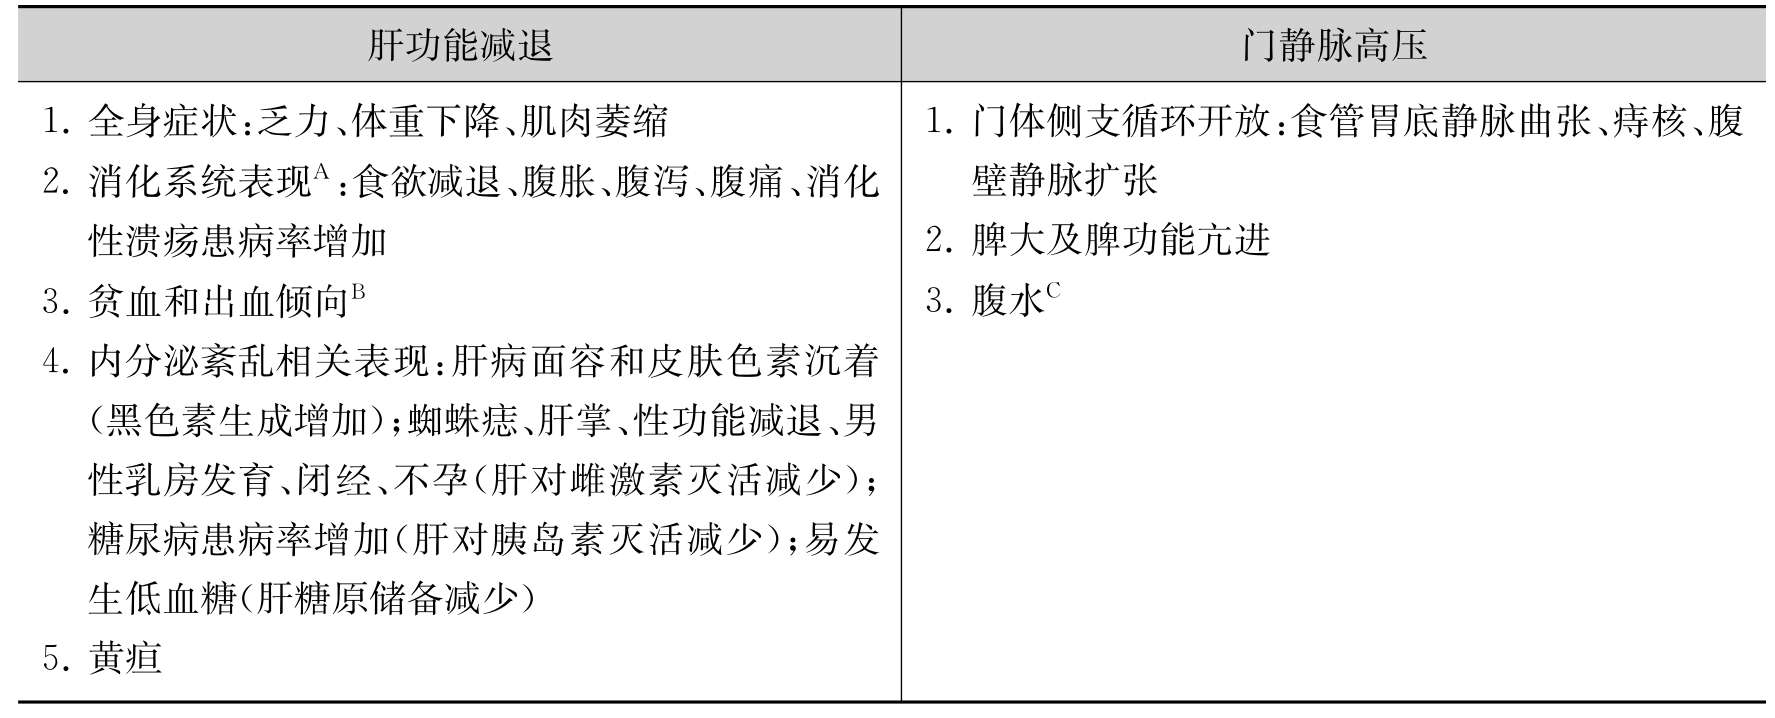
\includegraphics[width=5.90625in,height=2.38542in]{./images/Image00158.jpg}
\end{table}

失代偿期肝硬化诊断并不困难,依据下列各点可作出诊断:①有病毒性肝炎、长期大量饮酒等可导致肝硬化的有关病史;②有肝功能减退和门静脉高压的临床表现;③肝功能试验有血清白蛋白下降、血清胆红素升高及凝血酶原时间延长等指标提示肝功能失代偿;④B超或CT的辅助诊断,以及内镜发现食管胃底静脉曲张。代偿期肝硬化的临床诊断常有困难,对慢性病毒性肝炎、长期大量饮酒者长期密切随访,注意肝脾情况及肝功能试验的变化,如发现肝硬度增加,或有脾大,或肝功能异常变化,B超检查显示肝实质回声不均等变化,应注意早期肝硬化,必要时肝穿刺活检可获确诊。

在肝硬化的病因学鉴别诊断中应注意的一些问题:有些少见的遗传代谢性疾病(如肝豆状核变性)常易漏诊,已如前述;慢性缩窄性心包炎可引起肝大、腹水,如不注意会误诊为肝炎肝硬化;Budd-Chiari综合征常有明显门脉高压表现如脾大、腹水、腹壁静脉曲张及食管胃底静脉曲张,常被误诊为隐源性肝硬化。这些疾病均有明显肝大、病情与常见病因的肝硬化(如肝炎肝硬化和酒精性肝硬化)失代偿期肝功能试验的异常程度常不平行,此时应考虑这些少见疾病,相应检查多可鉴别(详见有关章节)。鉴别的重要意义在于这些疾病如能及早解除病因,病情多可恢复。

血吸虫病性肝硬化与肝炎肝硬化或酒精性肝硬化不论在病理学上与临床上均有差别。血吸虫病性肝硬化引起门静脉高压症状常较早和较重,脾大的发生率较多,巨脾症也多,食管与胃底静脉曲张破裂出血较多见。另一方面,平均发病年龄较轻,肝功能损害常较门脉性肝硬化为轻,因上消化道大出血而诱发肝性脑病的也较少见,因此,患者在脾切除术与门脉分流术后,预后也较门脉性肝硬化为好。此外,并发原发性肝癌者也较门脉性肝硬化为少。

\subsubsection{附:原发性胆汁性肝硬化}

原发性胆汁性肝硬化(PBC)病因未明,发病与免疫机制有关。罹患大多为中年妇女,起病缓慢,最常见的首发症状为无黄疸的皮肤瘙痒。常在黄疸发生前数月至两年出现瘙痒。黄疸亦可与皮肤瘙痒同时出现,但很少先有黄疸然后才有皮肤瘙痒。中年女性,有皮肤瘙痒,特别是不伴有黄疸,而有血清碱性磷酸酶活性增高,应考虑PBC的可能。

体检发现肝脾大,色素沉着常见。黄疸患者并发症可有脂肪泻、低血钙、高胆固醇血症、脂溶性维生素缺乏症、病理性骨折等。血清抗线粒体抗体(AMA)阳性率为84\%~96\%,对本病有诊断价值。B超、CT、ERCP有助于明确肝外胆管有无阻塞,有鉴别诊断意义。

中年妇女,起病徐渐,主诉皮肤瘙痒,伴有或不伴有黄疸,体检肝脾大,实验室检查符合胆汁淤积性黄疸,血清AMA阳性,滴度常在1∶128以上,具有特征性意义,或伴血清IgM增高,肝活检符合PBC的组织学改变,可确诊为原发性胆汁性肝硬化。

原发性与继发性胆汁性肝硬化均可并发黄色瘤,有人称为黄色瘤胆汁性肝硬化。此病临床上少见,国内仅有少数病例报告。发病在30~50岁之间,几全为女性。黄色瘤可分为斑状与结节状两种。前者好发于眼睑;后者好发于四肢的伸侧,尤以肘关节的伸侧多见,呈对称性分布。

\subsection{107.6 肝肿瘤与肝囊肿}

\subsubsection{一、原发性肝癌}

原发性肝癌在国内的发病率甚高,尤以华东与华南地区。发病年龄多在31~50岁之间。大批病理材料显示:肝细胞癌占82.9\%,胆管细胞癌11.5\%,混合细胞癌5.6\%;男性发病显著高于女性(8.54∶1),与病毒性肝炎及肝硬化多见于中青年男性有关。

起病缓慢,早期症状常不明显,不少患者因进行性消瘦、食欲不振而就诊,体检方发现肝大。凡年龄在30岁以上的男性患者,有进行性消瘦,肝大而硬、呈结节状,或兼有右季肋部疼痛者,须考虑原发性肝癌。此病多发生于肝硬化基础之上,两者的硬度与表面情况相似,但如患者无黄疸而血清γ-谷氨酰转肽酶活性明显增高,则有利于原发性肝癌的诊断。甲胎蛋白(AFP)现已广泛用于肝细胞癌的普查、诊断、判断治疗效果、预测复发。肝细胞癌AFP阳性率为70\%~90\%。在生殖腺胚胎瘤、少数转移性肿瘤如胃癌以及孕妇、肝炎、肝硬化、AFP可呈假阳性,但升高不如肝癌明显。目前多用放射免疫法(RIA)或AFP单克隆抗体酶免疫(EIA)快速测定法检测。两者方法灵敏、准确、便捷,无需特殊设备,适于普查。AFP浓度通常与肝癌大小呈正相关。在排除妊娠、肝炎和生殖腺胚胎瘤的基础上,AFP检查诊断肝细胞癌的标准为:①AFP大于500μg/L持续4周;②AFP由低浓度逐渐升高不降;③AFP在200μg/L以上的中等水平持续8周。

活动性慢性肝炎和肝硬化病例有20\%~45\%的AFP呈低浓度阳性,多不超过200μg/L,常先有血清ALT(GPT)明显升高,AFP呈同步关系,一般在1~2个月内随病情好转、ALT下降而下降。如AFP呈低浓度阳性持续达2个月或更久,ALT正常,应特别警惕亚临床肝癌的存在。

AFP异质体,临床上常遇到良性肝病的AFP值明显升高(>400μg/L)或原发性肝癌的AFP值偏低(<400μg/L),因此根据血清AFP浓度难以鉴别良恶性肝病。近年采用扁豆凝集素(LCA)亲和双向放射免疫电泳方法检测,显示人体血清AFP可分成LCA结合型和LCA非结合型两种AFP异质体。两者同时存在但各占总量的比值因病而异。在肝癌血清中结合型比值高于25\%,而在良性肝病中,结合型比值均低于25\%。根据两型异质体的比值可鉴别良恶性肝病,对肝癌的诊断率为87.2\%,假阳性仅2.5\%,且诊断不受AFP浓度、肿瘤大小和病期早晚的影响。

AFP单克隆抗体,选用针对LCA结合型AFP的单克隆抗体建立特异性强、灵敏度高的方法,或将抗体用核素标记,可有助于鉴别肝癌和良性肝病以及肝癌的定位。

当肝癌细胞脱落在循环迁移过程中可从周围血中测出AFPrnRNA,可用于预测肿瘤的复发和转移。

在AFP阴性的原发性肝癌,可联合检测γ-谷氨酰转肽酶同工酶Ⅱ(γ-GTⅡ)、异常凝血酶原、岩藻糖苷酶(AFU)等,可提高诊断阳性率。

肝癌的定位诊断,各种影像学检查方法依次为:肝动脉造影1~2cm直径,CT≤2cm,B超灰阶扫描2~3cm,放射性核素肝扫描3~5cm。选择性肝动脉造影国内报告成功率达96\%,且能发现直径1cm的小肝癌,诊断价值大,但为侵入性检查方法。CT和MRI为非侵入性检查法,临床较常应用。近年来发展的正电子发射计算机断层显像(PET)对诊断和鉴别诊断有重要价值。也可用B超或CT引导下肝穿刺活检进行诊断。

\subsubsection{二、继发性肝癌}

肝内转移癌最多起源于胃、肠、胰腺、子宫、卵巢、前列腺、膀胱、乳房、肺与腹膜后组织的癌。确诊须发现原发癌与肝内转移癌的存在。肝内转移癌通常为多数性,触诊可发现肝大而质硬,常有数量不定的大小结节,呈弥漫性浸润者甚少。碱性磷酸酶、乳酸脱氢酶、γ-谷氨酰转肽酶活性在相当早期可有较明显的增高。B超、CT、MRI、PET等影像学检查方法对鉴别原发性肝癌和继发性肝癌以及发现继发癌灶有重要意义。但也有少数患者可始终不能发现原发癌灶。

\subsubsection{三、其他肝脏肿瘤和囊肿}

\paragraph{(一)肝囊肿}

肝囊肿是指先天性、非寄生虫性肝囊肿;可单发或多发,常合并其他脏器的囊肿。囊肿可孤立单发也可局限累及一叶或弥漫性累及全肝,囊肿大小不等,大者可达数十厘米,小者如针尖。多数患者囊肿发展非常缓慢或发展至一定程度即停止。但少数人虽缓慢生长,最终压迫周围脏器而产生症状。肝囊肿近半数合并肾囊肿,部分多囊肝合并胰腺囊肿,合并脾囊肿者极少。

临床表现:本病女性多见,大多无明显症状,全身情况良好,有症状者多在40~50岁时出现。有症状者多呈上腹胀,部分伴有右上腹隐痛、肝区不适、消化不良症状,或以上腹部肿物为首发症状。

并发症:少见。囊内出血肝区疼痛加重,囊肿急剧增大,但多为小量出血。囊肿破裂致腹膜炎,囊液对腹膜刺激较轻微,故腹膜刺激征不明显。囊肿继发感染多发性弥漫性囊肿至晚期常发生门脉高压、腹水、胸水以及肝衰竭。个别孤立性囊肿有报道发生癌变,特别是囊壁有不规则结节时应疑及癌变。

辅助检查:B超检查是当前最有效而无创伤的一种检查方法,它能确定病灶大小、数量,分布部位,并能与肝外囊肿、寄生虫性囊肿以及病灶液化相鉴别,同时发现是否伴有肾、胰、脾等脏器囊肿。腹部平片检查可见肝影增大,如囊肿位于肝膈面,可见到局限性膈肌膨出或抬高。CT检查也是有效的诊断方法,显示囊肿大小、形状、部位,及有无合并其他脏器囊肿,能确定病灶的性质。MRI检查诊断价值同CT、B超检查。核素检查可以定位,但不能鉴别囊肿性质,且囊肿小者不能发现,其诊断价值不如B超和CT。通过病史、体检、特殊检查,诊断多无困难。

\paragraph{(二)肝海绵状血管瘤}

肝脏血管瘤比其他内脏的血管瘤为多见,其中尤以海绵状血管瘤为多。可发生于任何年龄,常在成年出现症状,女性多见。国内报道以单发性血管瘤为多,分布似以左叶为多。最常见的体征为上腹部包块。起病缓慢,病程长,体积小者无症状,常在B超检查时偶然发现。部分的海绵状血管瘤逐渐增大,形成右上腹包块,可被触及,并使人感觉肿块来自肝脏。病灶大于5cm时可伴腹部不适、肝大、消化不良等。肝功能一般正常。血窦中的血量可增加或减少,故肿块可有暂时性缩小,有时在肿块上可听到静脉营营音,用手压之此音可明显减弱或消失,是此瘤可靠的阳性征。肝功能试验大致正常。此瘤可被误诊为肝硬化、肝癌、肝包虫病、胰腺囊肿及胃癌等。B超、CT、MRI有助于诊断和鉴别诊断。血管瘤穿刺活检可导致严重出血,属禁忌。如临床上遇见病程长、全身情况良好、发展缓慢的上腹部肿块,须注意血管瘤的可能性。

此瘤迅速增大引起自发性出血时,可突然发生剧烈上腹痛与休克,易误诊为其他急腹症,往往须经剖腹探查方能明确诊断。

\paragraph{(三)原发性肝肉瘤}

本病少见,近年国内报道一组8例,年龄17~60岁,均以右上腹部隐痛或胀痛和右上腹肿块为主要临床表现。影像学检查均提示肝内占位性变,但术前定性诊断困难,致全部病例均误诊。由于此瘤体积多较大,常有中心部组织坏死、液化形成囊腔,影像学检查易误诊为肝囊性病变。早期手术切除肿瘤,可望提高生存率。

\paragraph{(四)肝母细胞瘤}

肝母细胞瘤是一种肝脏的胚胎性恶性肿瘤。其病因和发病机制目前尚不清楚,可能与染色体基因变异有关。临床表现:本病最常见于儿童期。文献报道5岁以下患儿占90\%,平均年龄16个月,男女比为2∶1。本病的主要临床表现为右上腹肿块并呈进行性增大,体检肝大可扪及质坚肿块。若出现明显症状和体征,包括发热、消瘦、贫血、食欲不振、黄疸、体重下降等常提示处于晚期。罕见情况下肿瘤细胞分泌HCG,导致青春期早熟、出现阴毛、生殖器增大以及声音变粗,多发生于男孩。诊断:血AFP升高。AFP水平与疾病过程平行,当肿瘤完全切除时,AFP降至正常而随病变复发,AFP水平可再度升高。可有其他实验室指标异常包括血清胆固醇、胆红素、碱性磷酸酶以及天冬氨酸转移酶水平的升高。CT可显示肝内单个或多个肿物,50\%病例有钙化灶。MRI及CT有助于将肝母细胞瘤与婴儿型血管内皮瘤、间叶性错构瘤等相区别。MRI还可显示肝母细胞瘤的上皮及间叶成分。

\paragraph{(五)肝细胞腺瘤}

肝细胞腺瘤是一种少见的肝细胞来源的良性肿瘤,通常由类似正常肝细胞组成。近年国外报道认为与口服避孕药有密切关系。在口服避孕药问世之前,本病极为罕见。而20世纪70年代以后随着类固醇激素避孕药的广泛应用,本病的发病率明显增高。肝细胞腺瘤由于生长缓慢常无特征性症状,随着肿瘤逐渐增大可出现腹胀、隐痛等压迫症状。有17.2\%~30\%的患者由于外伤造成瘤体破裂或瘤内自发性破裂导致腹腔大出血,出现失血性休克,甚至死亡。本病术前诊断较难,容易与肝癌相混淆诊断主要依据影像学检查,尤以CT检查最具价值。B超检查可见肝内孤立的圆形、椭圆形、边界清楚的低回声或中等回声肿块,肿瘤较大则回声杂乱、强弱不等。CT平扫呈圆形稍低密度,与周围肝组织相差10Hu,病灶边界清楚,有包膜,其内有更低密度的陈旧性出血、坏死灶增强扫描早期可有短暂的均匀性增强,和正常肝组织对比十分明显,然后密度下降为等密度,延迟扫描为低密度。

\paragraph{(六)肝错构瘤}

肝错构瘤是一种极罕见的肝脏先天性肿瘤样畸形。该肿瘤常见于肝脏创伤或穿刺后,近年来有人认为与口服避孕药有关,病因一直不清楚。可能与肝细胞酶系统缺损、激素类药物的刺激、肝细胞坏死后再生有关。本肿瘤多见于婴幼儿,男性多于女性,成人极罕见。早期无任何症状,少数病例为尸体解剖时偶然发现,绝大多数病例以腹围进行性增大或上腹部触及质硬肿块为主要临床特点。当肿瘤增大压迫邻近器官时,可出现恶心、呕吐、腹胀、黄疸、腹水等。肿块可随呼吸上下移动,通常无压痛。腹部X线平片、放射性核素扫描、血管造影、B超及CT等辅助检查对诊断有一定帮助。但易与肝母细胞瘤、神经母细胞瘤、肝癌、肝血管瘤和淋巴管瘤等相混淆。确诊须依据剖腹探查做病理检查或细针穿刺细胞学检查。

\paragraph{(七)肝脂肪瘤}

肝脏脂肪瘤罕见,多见于肥胖者。其由脂肪组织构成,周围可有完整的薄层纤维组织包膜,瘤体有成群的正常脂肪细胞被纤维组织束分成叶状,有的脂肪瘤可有较多的纤维组织随着肝脏显像技术的进步和肝脏外科的迅速发展,这种肝脏良性肿瘤的发现可能会有所增加。肝脂肪瘤一般无症状,多在体检时被B超、CT检查发现,B超图像表现为极强的回声光团,光点特别细小、致密,内有血管通过。边缘锐利,略有分叶感,整个图像类似个“太阳球”;CT检查有其特征性表现:即脂肪瘤的吸收系数为负值。本病治疗以手术切除为主,对确诊的较小脂肪瘤可暂观察,如有明显增大,可再手术治疗。脂肪瘤不会恶变,预后良好。

\subsubsection{四、肝脏炎性假瘤}

肝脏炎性假瘤少见。发病机制不明。本病以一个(也有多发)包块的形式发生于肝内。多数病变为有包膜的实性肿物,多呈圆形或椭圆形,直径大小1~25cm,病程长,多为有症状时经B超检查发现。症状无特异性,主要临床表现为原因不明的发热、右上腹部疼痛、体重减轻、黄疸、右上腹包块等。肝功能可有轻度异常。绝大多数AFP阴性,也有少数呈阳性。AFP阳性机制未明,可能与肝细胞增生有关。超声、CT、MRI对病灶定位很有价值,但一部分患者不能准确显示病变性质,易误诊为肝癌。B超引导下细针穿刺活检是有效的定性诊断方法。手术切除是主要治疗方法。

\subsubsection{五、肝脏结节性再生性增生}

肝脏结节性再生性增生罕见,发病年龄为8~81岁,以50岁中年患者多见。病因未明。病理特点为多发性小结节弥漫分布于全肝。临床表现差别甚大,从无症状乃至严重的门脉高压症。是引起非硬化性门脉高压症的主要原因。半数伴有门脉高压。超声可呈等回声,在多个小回声肿物中如出现无回声的中心区,则可能为小结节内出血。CT显示为一个或多个低密度区。核素肝脏扫描显示多个分散小肿物,有诊断价值。开腹探查见肝表面布满大小1~3mm的苍白至褐黄色小结节,膨出肝表面,边界清楚,无包膜。病理活检可确诊。可B超引导下穿刺或腹腔镜直视下取活检。

\subsection{107.7 血液病性肝大}

红细胞系统病变,如真性红细胞增多症、阵发性睡眠性血红蛋白尿、蚕豆病、血红蛋白病、遗传性铁粒幼细胞性贫血等均可引起轻重程度不同的肝大。白细胞系统病变,如白血病、恶性淋巴瘤、多发性骨髓瘤、恶性组织细胞病等均可导致肝损害、肝大。上述疾病所致肝大均有原发病的表现。

\subsection{107.8 结缔组织病性肝大}

本病有肝功能异常者不多见,仅系统性红斑狼疮、结节性多动脉炎、类风湿关节炎的某些类型、系统性硬化、干燥综合征及多发性风湿肌病有轻度肝大。如系统性红斑狼疮约1/3病例有肝大,肝功能异常表现为转氨酶升高,偶有AKP及胆红素增高。大部分发生在SLE的活动期。类风湿关节炎伴Felty综合征者,有脾大及粒细胞减少、肝脏有结节增生。干燥综合征有多种组织和器官抗体的自身免疫现象,可有抗核抗体、壁细胞抗体、抗甲状腺抗体阳性等。

类狼疮性肝炎(lupoid
hepatitis)是一种特别类型的活动性慢性肝炎伴有系统性红斑狼疮的表现,病情常严重,预后不佳,最后发展为坏死后性肝硬化。患者几全为女性,临床表现与系统性红斑狼疮相符,但肝脏方面的表现较为突出,有肝、脾大与明显的肝功能损害,其他症状为多发性关节炎、胸膜炎、血小板减少性紫癜、血沉加快、血清丙种球蛋白增加、蛋白尿、镜下血尿、血中出现狼疮细胞等。目前公认本病是以肝脏损害为主的系统性红斑狼疮,是系统性红斑狼疮的特别类型。

\protect\hypertarget{text00243.html}{}{}

\section{参考文献}

1.中华医学会传染病与寄生虫学分会、肝病学分会.病毒性肝炎防治方案.中华肝脏病杂志2000,8(6):324

2.陆志檬.丙型肝炎的临床特征和血清、病毒学试验.胃肠病学,2002,7(6):360

3.杨柳明,等.肝活检对转氨酶正常的慢性乙型肝炎感染的临床意义.中华消化杂志,2001,21(10):590

4.覃肇源,等.儿童传染性单核细胞增多症的肝损害和心肌酶异常.新医学,2005,36(10):580

5.孙经利,等.巨细胞病毒性肝炎四例.临床肝胆病杂志,2005,21(1):6

6.刘庆全.细菌性肝脓肿90例临床诊治体会.肝胆外科杂志,2002,4(10):116

7.刘思纯.肝胆胰感染性疾病的抗菌药物应用.新医学,2004,35(3):171

8.刘梅华,等.布-加综合征临床特点及治疗转归分析.中华消化杂志,2002,22(6):382

9.郑冬,等.前列地尔对造血干细胞移植中肝静脉闭塞病的预防作用.新医学,2003,34(5):296

10.张莉,等.肝小静脉闭塞症一例.中华内科杂志,2005,44(5):391

11.李堂,等.88例儿童肝豆状核变性临床分析.中华肝脏病杂志,2003,11(2):118

12.赵新颜,等.30例淀粉样变患者的临床特点分析.中华肝脏病杂志,2005,13(1):42

13.形迎红.肝移植治疗糖原贮积症一例.新医学,2002,33(6):356

14.杨绍基.肝硬化的临床分类与实验室检查.新医学,2002,33(3):182

15.王吉耀,等.原发性胆汁性肝硬化的临床及病理学特征.中华肝脏病杂志,2002,10(5):334

16.崔儒涛,等.异常凝血酶Ⅱ在肝细胞癌诊断价值的评价.中华消化杂志,2001,21(11):701

17.刘丽,等.超声在肝脏疾病中的应用.新医学,2001,32(11):695

18.钟崇,等.肝脏炎性假瘤18例临床特点与治疗探讨.新医学,2005,36(7):391

19.杨冬华,等.肝脏结节性再增生性增生的临床诊治.新医学,2001,32(2):119

20.张烜,等.96例系统性红斑狼疮的肝脏损害分析.中华内科杂志,1998,37(1):45

21.中华医学会肝病学分会脂肪肝和酒精性肝病学组.酒精性肝病诊疗指南(2010年修订版).中华肝脏病杂志,2010,18(3):167-170

22.中华医学会肝脏病学分会脂肪肝和酒精性肝病学组.非酒精性脂肪性肝病诊疗指南(2010年1月修订).中华内科杂志,2010,49(3):275-278

23.蒲从伦,郭春宝,金先庆,等.肝母细胞瘤患儿及其母亲孕期特点回顾性分析.中华肝脏病杂志,2009,17
(6):459-461

24.彭利,王顺祥,张风瑞,等.肝细胞腺瘤的诊断和治疗.中华肝胆外科杂志,2002,8(12):721-722

25.郭子军.肝错构瘤1例.中国医师进修杂志,2006,29(32):70

26.李金龙,李荣祥.肝脂肪瘤一例.中华肝胆外科杂志,2001,7(1):45

27.刘坤,林斌,汪启乐,等.细菌性肝脓肿影响因素分析.肝胆外科杂志,2012,20(1):40-42

28.贾国葆,周毅力,骆定海,等.肝结核的临床特点及诊治分析.中华临床感染病杂志,2010,03(5):280-282

29.顾青,王关顺,包颜明,等.肝梅毒的MRI表现一例.放射学实践,2006,21(2):206

30.杨光耀,丁志强,俞亚红,等.肝放线菌病一例.临床外科杂志,2011,19(5):340

31.董剑宏,宋炎阳,李小争,等.阿米巴肝脓肿74例治疗分析.中华传染病杂志,2000,18(4):273-274

32.于建武,孙丽杰,康鹏,等.华支睾吸虫病88例流行病学和临床特征分析.中华传染病杂志,2008,26(12):744-746

33.戴季蓬,邵英梅,温浩,等.肝包虫病的诊断与治疗进展.中华肝胆外科杂志,2011,17(5):432-433

34.黄正美,邢兰燕,范波,等.肝片吸虫病1例报告.中国热带医学,2006,6(9):1624

35.刘思纯,马博.药物性肝损害的诊断和治疗现状.新医学,2007,38(9):564-566

36.邱新运,于成功,钱铖,等.以肝大为特征的肝淀粉样变性1例.胃肠病学,2011,16(2):127-128

37.李光明,范建高.肝豆状核变性的诊断与治疗进展.实用肝脏病杂志,2012,15(6):493-495

38.申德林,焦栓林,朱晓红,等.肝糖原累积病13例误诊分析.中华消化杂志,2004,24(6):357

39.尧颖,徐智媛,高建鹏,等.60例原发性胆汁性肝硬化患者的临床与病理特征及预后分析.中华肝脏病杂志,2008,16(6):457-460

40.樊嘉,史颖弘.原发性肝癌研究:基础与临床的转化.中华肝胆外科杂志,2011,17(5):357-358

41.江建军,郭怀斌.多囊肝与单纯性多发肝囊肿的诊断与治疗.中国综合临床,2010,26(5):534-536

42.黄志强,黄晓强,张文智,等.肝海绵状血管瘤外科治疗20年的经验与反思.中华消化外科杂志,2009,8
(3):161-167

43.曹利平,胡均安,阙日升,等.成人原发性肝肉瘤四例诊治分析.中华普通外科杂志,2009,24(8):617-620

44.耿兴聪,史长涛,潘延涌,等.肝脏炎性假瘤诊治分析.中国临床实用医学,2010,04(10):215-216

45.中华医学会消化病学分会肝胆疾病协作组.急性药物性肝损伤诊治建议(草案).中华消化杂志,2007,27
(11):765-767

\protect\hypertarget{text00244.html}{}{}

